

\tikzset{every picture/.style={line width=0.75pt}} %set default line width to 0.75pt        

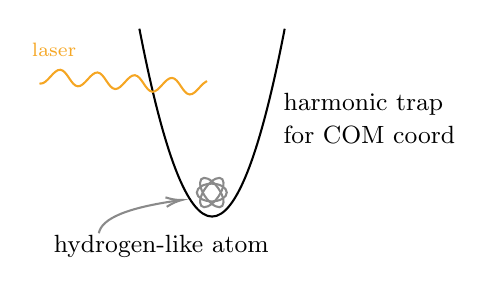
\begin{tikzpicture}[x=0.75pt,y=0.75pt,yscale=-1,xscale=1]
%uncomment if require: \path (0,126); %set diagram left start at 0, and has height of 126

%Shape: Parabola [id:dp6726865290868447] 
\draw   (57.33,1.49) .. controls (80.67,122.17) and (104,122.17) .. (127.33,1.49) ;
%Shape: Wave [id:dp7512032357045172] 
\draw  [color={rgb, 255:red, 245; green, 166; blue, 35 }  ,draw opacity=1 ] (9.18,27.82) .. controls (9.35,27.88) and (9.53,27.91) .. (9.71,27.93) .. controls (11.34,28.05) and (12.87,26.36) .. (14.47,24.6) .. controls (16.07,22.83) and (17.6,21.15) .. (19.22,21.27) .. controls (20.85,21.39) and (22.12,23.27) .. (23.44,25.25) .. controls (24.77,27.23) and (26.04,29.12) .. (27.66,29.24) .. controls (29.29,29.36) and (30.82,27.67) .. (32.42,25.91) .. controls (34.02,24.14) and (35.55,22.46) .. (37.17,22.58) .. controls (38.8,22.7) and (40.07,24.58) .. (41.39,26.56) .. controls (42.72,28.54) and (43.99,30.43) .. (45.62,30.55) .. controls (47.24,30.66) and (48.77,28.98) .. (50.37,27.22) .. controls (51.97,25.45) and (53.5,23.77) .. (55.13,23.89) .. controls (56.75,24) and (58.02,25.89) .. (59.35,27.87) .. controls (60.67,29.85) and (61.94,31.74) .. (63.57,31.85) .. controls (65.19,31.97) and (66.72,30.29) .. (68.32,28.52) .. controls (69.92,26.76) and (71.45,25.08) .. (73.08,25.19) .. controls (74.7,25.31) and (75.97,27.2) .. (77.3,29.18) .. controls (78.63,31.16) and (79.9,33.04) .. (81.52,33.16) .. controls (83.15,33.28) and (84.68,31.6) .. (86.28,29.83) .. controls (87.5,28.48) and (88.68,27.18) .. (89.9,26.7) ;
%Shape: Ellipse [id:dp06930515818625183] 
\draw  [color={rgb, 255:red, 138; green, 138; blue, 138 }  ,draw opacity=1 ] (85,80.41) .. controls (85,78.06) and (88.23,76.15) .. (92.21,76.15) .. controls (96.19,76.15) and (99.42,78.06) .. (99.42,80.41) .. controls (99.42,82.77) and (96.19,84.68) .. (92.21,84.68) .. controls (88.23,84.68) and (85,82.77) .. (85,80.41) -- cycle ;
%Shape: Ellipse [id:dp5001538841210537] 
\draw  [color={rgb, 255:red, 138; green, 138; blue, 138 }  ,draw opacity=1 ] (87.11,74.02) .. controls (88.44,72.35) and (91.8,73.87) .. (94.61,77.4) .. controls (97.43,80.93) and (98.64,85.15) .. (97.31,86.81) .. controls (95.98,88.48) and (92.63,86.96) .. (89.81,83.43) .. controls (86.99,79.89) and (85.79,75.68) .. (87.11,74.02) -- cycle ;
%Shape: Ellipse [id:dp5281934647928739] 
\draw  [color={rgb, 255:red, 138; green, 138; blue, 138 }  ,draw opacity=1 ] (87.11,86.81) .. controls (85.79,85.15) and (86.99,80.93) .. (89.81,77.4) .. controls (92.63,73.87) and (95.98,72.35) .. (97.31,74.02) .. controls (98.64,75.68) and (97.43,79.89) .. (94.61,83.43) .. controls (91.8,86.96) and (88.44,88.48) .. (87.11,86.81) -- cycle ;
%Curve Lines [id:da8270564180244198] 
\draw [color={rgb, 255:red, 138; green, 138; blue, 138 }  ,draw opacity=1 ]   (37.78,100.02) .. controls (39.06,93) and (51.13,87.76) .. (75.85,84.28) ;
\draw [shift={(77.78,84.02)}, rotate = 172.4] [color={rgb, 255:red, 138; green, 138; blue, 138 }  ,draw opacity=1 ][line width=0.75]    (7.65,-2.3) .. controls (4.86,-0.97) and (2.31,-0.21) .. (0,0) .. controls (2.31,0.21) and (4.86,0.98) .. (7.65,2.3)   ;

% Text Node
\draw (4,7) node [anchor=north west][inner sep=0.75pt]  [font=\scriptsize,color={rgb, 255:red, 245; green, 166; blue, 35 }  ,opacity=1 ] [align=left] {laser};
% Text Node
\draw (125.33,31) node [anchor=north west][inner sep=0.75pt]   [align=left] {{\small harmonic trap}\\{\small for COM coord}};
% Text Node
\draw (14.67,99.67) node [anchor=north west][inner sep=0.75pt]   [align=left] {{\small hydrogen-like atom}};


\end{tikzpicture}
